\begin{figure}[htb!]
  \begin{center}
    \resizebox{\textwidth}{!}{
      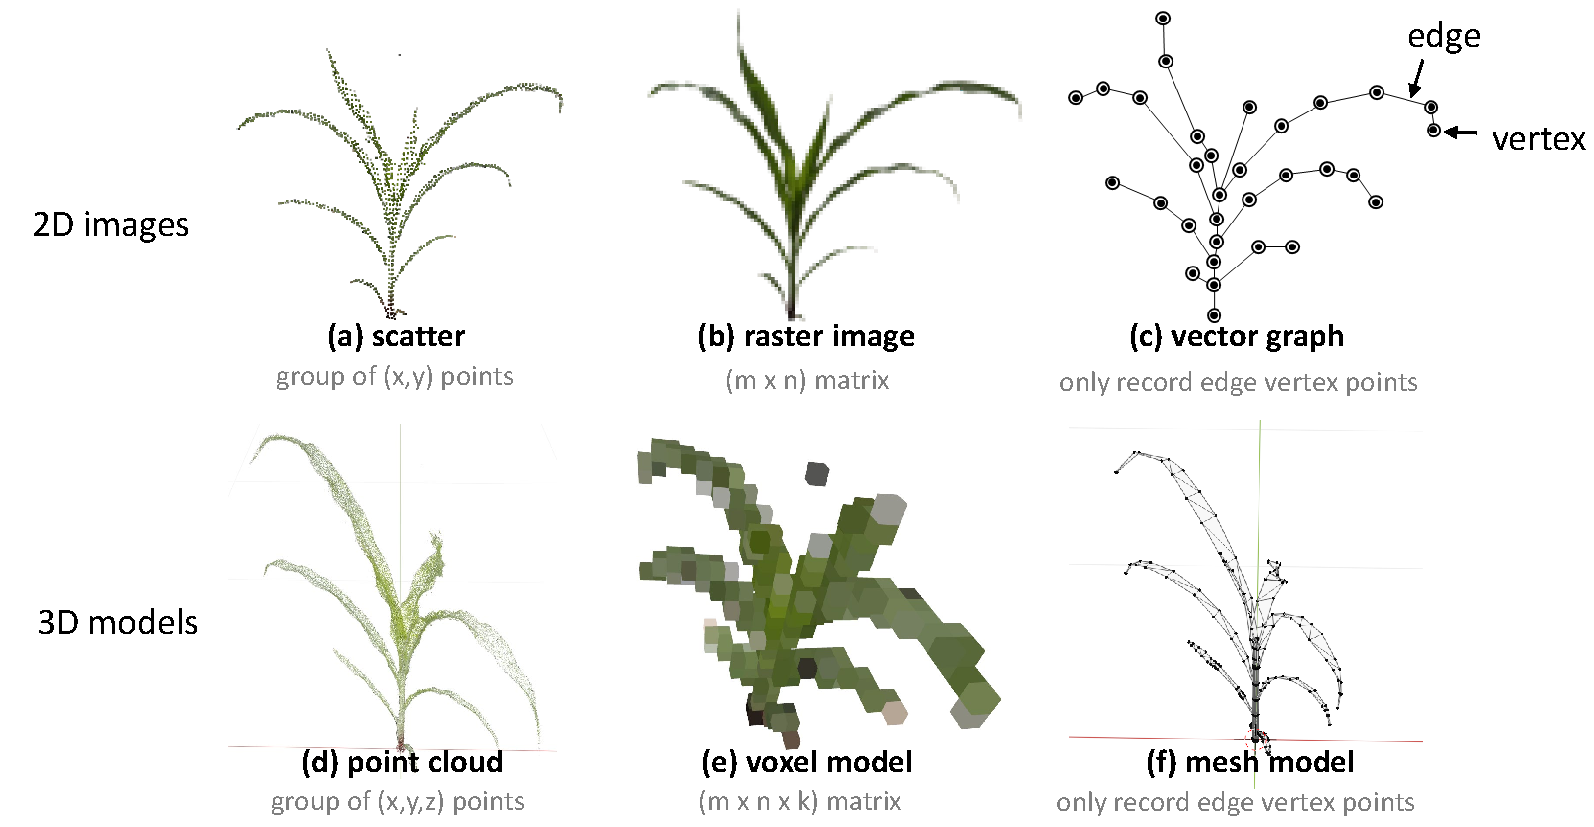
\includegraphics{figures/int/data_format.pdf}
    }
  \end{center}
  \caption[The compairson of 2D-based and 3D-based data format]{
    The comparison of 2D-based and 3D-based data format; (a) 2D point cloud also called scatter; (b) the common format for 2D images; (c) updated the scatter with relationship between points; (d) 3D point cloud, the most common format for 3D-based analysis; (e) the unit of 2D raster image is pixel, while the unit of 3D raster is voxel; (f) updated the point cloud with relationship, often used in \gls{cg} industry.
  }
  \label{fig:int3}
\end{figure}